\documentclass[a4paper, 12pt]{book}
\usepackage[a4paper, left=2.5cm, right=2.5cm, top=3cm, bottom=3cm]{geometry}
%\usepackage[a4paper]{geometry}
\usepackage{times}
\usepackage{color}
\usepackage[usenames,dvipsnames,svgnames,table]{xcolor}
\usepackage[utf8]{inputenc}
\usepackage[textwidth=2cm]{todonotes}
\usepackage[hyphens]{url}
\usepackage[english]{babel}
%\usepackage[dvipdfm]{graphicx}
\usepackage{float}
\usepackage{placeins}
\usepackage[nottoc, notlot, notlof, notindex]{tocbibind}
\usepackage{latexsym}  %% Logo LaTeX
\usepackage{graphicx}
\usepackage{multirow}
\usepackage[colorlinks,bookmarksopen]{hyperref}
\usepackage{booktabs}
\usepackage{etoolbox}
\makeatletter
\preto{\@verbatim}{\topsep=0pt \partopsep=0pt }
\makeatother

%\usepackage[svgnames]{xcolor}

\restylefloat{table}
\restylefloat{figure}

%% PDF metadata
\hypersetup{
  pdftitle={The OpenDaylight Open Source Project},
  pdfauthor={Sergio Najib Arroutbi Braojos},
  pdfcreator={Master on Libre Software (URJC), Universidad Rey Juan Carlos},
  pdfproducer=PDFLaTeX,
  pdfsubject={Libre Software},
  %%% change colors to darker ones (for printing in B/W)
  linkcolor=Sepia,
  citecolor=OliveGreen,
  filecolor=violet,
  urlcolor=blue
}
%%

% Alter some LaTeX defaults for better treatment of figures:
    % See p.105 of "TeX Unbound" for suggested values.
    % See pp. 199-200 of Lamport's "LaTeX" book for details.
    %   General parameters, for ALL pages:
    \renewcommand{\topfraction}{0.9}	% max fraction of floats at top
    \renewcommand{\bottomfraction}{0.8}	% max fraction of floats at bottom
    %   Parameters for TEXT pages (not float pages):
    \setcounter{topnumber}{2}
    \setcounter{bottomnumber}{2}
    \setcounter{totalnumber}{4}     % 2 may work better
    \setcounter{dbltopnumber}{2}    % for 2-column pages
    \renewcommand{\dbltopfraction}{0.9}	% fit big float above 2-col. text
    \renewcommand{\textfraction}{0.07}	% allow minimal text w. figs
    %   Parameters for FLOAT pages (not text pages):
    \renewcommand{\floatpagefraction}{0.7}	% require fuller float pages
	% N.B.: floatpagefraction MUST be less than topfraction !!
    \renewcommand{\dblfloatpagefraction}{0.7}	% require fuller float pages

\frenchspacing

\title{The OpenDaylight Open Source Project}
\author{Sergio Najib Arroutbi Braojos}

\renewcommand{\baselinestretch}{1.5}

\begin{document}

%\renewcommand{\refname}{Bibliography}
\renewcommand{\appendixname}{Appendix}

%%%%%%%%%%%%% COVER %%%%%%%%%%%%%%%%
\begin{titlepage}
\begin{center}
\begin{tabular}[c]{c c}
%
\includegraphics[bb=0 0 194 352, scale=0.25]{logo} &

\includegraphics[scale=0.25]{img/logo.png} &
\begin{tabular}[b]{l}
\Huge
\textsf{UNIVERSIDAD} \\
\Huge
\textsf{REY JUAN CARLOS} \\
\end{tabular}
\\
\end{tabular}

\vspace{3cm}

\Large
Máster Universitario en Software Libre

\vspace{0.4cm}

\large
Curso Académico 2014/2015

\vspace{0.8cm}

Proyecto Fin de Máster

\vspace{2.5cm}

\LARGE
The OpenDaylight Open Source Project

\vspace{4cm}

\large
Autor: Sergio Najib Arroutbi Braojos \\
Tutor: Dr. Gregorio Robles
\end{center}
\end{titlepage}
%%%%%%%%%%%%%%%%%%%%%%%%%%%%%%%%%%%%%%
\newpage
~

\newpage
~
\thispagestyle{empty}
\vspace{3cm}
\begin{flushright}
\textbf{\textit{Agradecimientos}} \\
\textit{A mi familia y a mi pareja, por su apoyo incondicional\\
Al equipo de Libresoft de la Universidad Rey Juan Carlos,
por su afán en enseñar el qué y el porqué del Software Libre}
\vspace{2cm}

\textbf{\textit{Dedicatoria}} \\
\textit{Para todos aquellos que hacen posible el fenómeno del Software Libre}
\end{flushright}

\newpage
~


\newpage
~
\thispagestyle{empty}
\vspace{12cm}
\begin{flushright}

(C) 2014 Sergio Najib Arroutbi Braojos. Some rights reserved.

This document is distributed under the Creative Commons
Attribution-ShareAlike 3.0 license,
available in \url{http://creativecommons.org/licenses/by-sa/3.0/}

Source files for this document are available at
\url{http://github.com/MFP/opendaylight.tex}
\end{flushright}

\newpage
~

\tableofcontents

\listoffigures

\listoftables

%%%%%%%%%%%%%%%%%%%%%%%%%%%%%%%%%%%%%%

\chapter*{Summary}
\markboth{SUMMARY}{SUMMARY}
\label{chap:summary}

The main goal of this work is to perform a deep analysis about the OpenDaylight Open Source Project. This collaborative project, hosted by the Linx Foundation, has been created in order to achieve one mission: \textbf{Develop an Open Source Programmable Networking Platform}.

In this document, a detailed study of the different Open Source aspects having to do with project of this type of characteristics will be analyzed. Examples of this aspects, are, for instance, the licensing mechanism adopted by the project, the community behind the project, descriptive statistics about the project, the economic aspects around the project, as well as the technical state of the proyect and how OpenDaylight has progressed from its foundation date.


\chapter*{Resumen}
\markboth{RESUMEN}{RESUMEN}
\label{chap:resumen}

El principal objetivo de este trabajo es realizar un análisis detallado del projecto de código abierto OpenDaylight. Este proyecto colaborativo, perteneciente a la Linux Foundation, ha sido creado para una misión principal: \textbf{Desarrollar una plataforma de Código Abierto para Redes Programables}.

En este documento, un estudio pormenorizado de los distintos aspectos asociados al Código Abierto asociados para un proyecto de estas características serán analizados. Un ejemplo de los aspectos a estudiar será el mecanismo de sistema de licencias, la comunidad que reside detrás del proyecto, estadísticas descriptivas del proyecto, los aspectos económicos, si los hubiera, alrededor del proyecto, así como el estado a nivel técnico o cómo ha evolucionado OpenDaylight desde la fecha de su fundación.

%%%%%%%%%%%%%%%%%%%%%%%%%%%%%%%%%%%%%%

\chapter{Introduction}
\label{chap:introduction}

\section{Terminology}
\label{sec:terminology}

\subsection{Open Source Programmable Networking}
\label{subsec:freesoftware}
In the same way Cloud Computing means a revolution in Computer Science, where computing resources are considered as flexible facilities to provide different kind of services, Networking is evolving in the same way. Networks hardware is considered to be a resource that is flexible and easily programmable in order to adapt to the specific Networking necessities. \textbf{SDN} (Software Defined Networking) and \textbf{NFV} (Network Functions Virtualization) ~\cite{SDN} technologies have been strongly brougth to foreground in Networking Science, in order to provide,on the one hand, management of the network services through abstraction of lower level functionality and characteristics, and, on the other hand to provide a network architecture virtualization technologies to simulate nodes exisiting on a network.\\
\\
Around these technologies, The OpenDaylight Open Source Project, hosted by the Linux Foundation, has appeared to provide mechanisms not only to use previous described technology, but also to guarantee all the potential users of this technology the Freedoms that Open Source means, i.e.:
\begin{itemize}
 \item Freedom to use the program, for any purpose
 \item Freedom to study and adapt the programs (modify)
 \item Freedom to distribute the program to others
 \item Freedom to distribute to others the modified versions of the program
\end{itemize}
Analyzing The OpenDaylight Open Source Project is a good oportunity to investigate, on the one hand, an incipient technology and how an also incipient Open Source Project can influence not only on that technology, but also on the different aspects around a technology, as people involved on the technology develeopment (Community), the impact on the Economic aspects around the technology, and, above all, the aspects that Open Source itself supposes for this kind of projects.

\section{About this document}
\label{sec:about}

\subsection{Document structure}

In order to provide a detailed analysis of The OpenDaylight Open Source Project, this work contains different chapters to describe the different important aspects aroud the project from an Open Source perspective:

\begin{table}[H]
\footnotesize
\begin{center}
\begin{tabular}{|p{5cm}|p{10cm}|}
\hline
\textbf{Chapter Name} & \textbf{Description} \\ \hline
Introduction & A complete introductory overview of The OpenDaylight Open Source Project \\
\hline
OpenDaylight Legal Aspects & Complete analysis of the license or licenses used in OpenDaylight and the different advantages and disadvantages of this kind of licensing scheme \\
\hline
OpenDaylight Economic Aspects & Detailed study of economic aspects around the project \\
\hline
OpenDaylight Technical Aspects & Study of the technology behind the project and its scope \\
\hline
OpenDaylight Governance and Community Management & Analysis of the community and its governance, its organization, communication channels, politics and mission  \\
\hline
OpenDaylight Project Evaluation & Graphics and statistics around the OpenDaylight project, such as number of commiters, number of open/closed issues, mail lists statistics, activity and in general all statistics to perform an evaluation of the project from a statistical perspective \\
\hline
\end{tabular}
\end{center}
\caption{Document Structure}
\label{tab:documentstructure}
\end{table}

\subsection{Scope}
\label{subsec:scope}
This document is not entitled to perform a complete description of the different protocols and technologies that OpenDaylight uses in order to achieve the programmability network platform it pretends to provide. They will be smoothly analyzed in order to clarify how OpenDaylight works, but not all of the technologies will be described, and those described will not be done in deep.

Beyond the purely technical aspects, this work pretends to focus on analyzing OpenDaylight project from an Open Source perspective, analysing the pros and cons of Open Source, and the different aspects that an Open Source Project faces.

\subsection{Methodology}
\label{subsec:methodology}
Different tools and documentation have been used in order to perform this work. Docmentation used have been basically the different Web Pages available around The OpenDaylight Open Source Project~\cite{OpenDaylight}. A complete description of the documentation used will be provided in the Bibliography.

Regarding tools, apart from Web-Browsers used to navigate through the project documentation, the different metrics obtained around OpenDaylight project have been obtained through MetricsGrimoire~\cite{MetricsGrimoire}. In particular, among the tools existing on MetricsGrimoire, CVSanaly~\cite{CVSanaly}, Bicho~\cite{Bicho} and MailingListStats~\cite{MailStats} were used.

%%%%%%%%%%%%%%%%%%%%%%%%%%%%%%%%%%%%%%
\chapter{Goals and Objectives}
\label{chap:Goals}
\section{General Objectives}
\label{sec:genobj}

The general objectives of this work are, basically, on the one hand, acquiring knowledge, competence and skills around OpenDaylight, while, on the other hand, analysing the project from an Open Source perspective.

\section{Subobjectives}
\label{sec:subobj}

%%%%%%%%%%%%%%%%%%%%%%%%%%%%%%%%%%%%%%
In order to achieve the objectives this work pursues next operative objectives have been identified:

\begin{itemize}
\item{Acquire competence on OpenDaylight project}
\item{Analyze OpenDaylight project from an Open Source perspective}
\item{Extract the most significant statistics in OpenDaylight project to determine its state of the art}
\end{itemize}

\subsection{Acquire competence on OpenDaylight project}
\begin{itemize}
 \item Perform an overall description of the OpenDaylight project.
 \item Acquire competence on OpenDaylight documentation, and sinthesize the most important aspects of the project.
 \item Analyze the technical aspects of the project and determine its Ease of Use.
\end{itemize}

\subsection{Analyze OpenDaylight project from an Open Source perspective}
\begin{itemize}
 \item Analyze the licensing model followed by the project
 \item Study the economic aspects behind this project
 \item Determine the different aspects behind the project's community
\end{itemize}

\subsection{Statistics and measures of the OpenDaylight project}
\begin{itemize}
 \item Perform a complete measures compilation of the project
 \item Evaluate the State of the Art of the project based on its measures
\end{itemize}

\chapter{OpenDaylight: A first view}
\label{chap:odlfirstview}

\section{OpenDaylight Project}
\label{sec:odlintro}

OpenDaylight is a collaborative project, started in April 8, 2013~\cite{OpenDaylightAnnouncement}, and developed inside the Linux Foundation Collaborative Projects ecosystem. This fact is the first one to remark, due to the fact that, normally, projects under the Linux Foundation are supposed to have strong economic and infrastructure support, due to the following reasons:
\begin{itemize}
 \item \textbf{Linux Foundation} is one of the most profitable Open Source organizations, mostly due to the importance of its main project, \textbf{the Linux Kernel Project}. In 2012, The Linux Foundation obtained a \textbf{total revenue of \$17,123,662}, according to ~\cite{2012LinuxFoundationReport}. Among the collaborators of the Linux Foundation Collaborative Projects, next ones are to remark: ~\cite{LinuxFoundationCollaborativeProjects}
 \begin{enumerate}\itemsep0pt
  \item Cisco
  \item Google
  \item HP
  \item IBM
  \item Intel
  \item Qualcomm Innovation Center
  \item Samsung
  \item New York Stack Exchange Technologies
 \end{enumerate}
 \item \textbf{Collaborative Projects} under the Linux Foundation are only a few, in a more focused strategy compared to other organizations hosted in other organizations such as Mozilla Foundation, the Apache Software Foundation or the Free Software Foundation, that fund more projects. Examples of other projects hosted by the Linux Foundation Collaborative Projects are ~\cite{LinuxFoundationCollaborativeProjects}:
 \begin{enumerate}\itemsep0pt
  \item Allseen Alliance
  \item Code Aurora
  \item MeeGo
  \item OpenVirtualization Alliance
  \item The Bel Language
  \item OpenMama
  \item Tizen
  \item Xen Project
  \item Yocto Project
 \end{enumerate}
\end{itemize}
Being a Linux Foundation Collaborative Project, OpenDaylight is part of a technology that is booming in the last years, having to do with \textbf{SDN} and, to a lesser extent, with NFV, in particular in the Networking Industry. According to OpenDaylight project ~\cite{OpenDaylightTheProject}:
\begin{verbatim}
OpenDaylight is a community-led, open, industry-supported
framework, for accelerating adoption, fostering new innovation,
reducing risk and creating a more transparent approach to
Software-Defined Networking.
OpenDaylight is a Collaborative Project at The Linux Foundation.
It is structured using open source development best practices,
and is comprised of the leading organizations in the technology
industry.
\end{verbatim}
In particular, as stated in the ``About'' section of OpenDaylight project~\cite{OpenDaylightAbout}, the adoption of new technologies and pursuit of programmable networks has the potential to significantly improve levels of functionality, flexibility and adaptability of mainstream datacenter architectures.\\
\\
Leveraging this abstraction to its fullest requires some adaptation from the network perspective, as well as adaptation and evolution to a Software-Defined architecture. One of the most important architectural elements required to achieve this goal is SDN and NFV platform, to enable network control and programmability from a centralized point.\\
\\
SDN, and NFV to a lesser extent, are a hotbed of innovation nowadays, with a bunch of vendors bringing products and technologies to market. Ironically, the myriad options may prove counterproductive to SDN and NFV adoption. At this early stage of SDN and NFV adoption, the industry acknowledges the benefits of establishing an open, reference framework for programmability and control through an open source SDN and NFV solution.\\
\\
Such a framework maintains the flexibility and choice for organizations to deploy SDN and NFV as they still mitigates many of the risks of adopting early stage technologies and integrating with existing infrastructure investments.\\
\\
With OpenDaylight, a community with some of the most important companies involved in Computer Science, Virtualization and Networking Industry, has come together to fill this need through the combination of open community developers and open source code and project governance that guarantees an open, community decision making process on business and technical issues. \textbf{Establishing an open source project in this way is designed to help accelerate the development of technology available to users} and enable widespread adoption of SDN and create a solid foundation for NFV.\\
\\
OpenDaylight can be a \textbf{core component} within any SDN architecture, providing an open source SDN and NFV controller that enables users to reduce operational complexity, extend the life of their existing infrastructure hardware and enable new services and capabilities only available with SDN.\\
\\
Whether an organization is an enterprise IT provider, a network service provider or a Cloud services provider, it can begin taking advantage of SDN and NFV using a community-driven, open source controller framework available today.\\
\\
The first open source software release by the OpenDayLight Open Source Project is known as \textbf{``Hydrogen''}. This release, Hydrogen, is the first simultaneous release of OpenDaylight, delivering three different editions to help a wide array of users get up and running as quickly as possible. The three options available are a Base Edition, a Virtualization Edition and a Service Provider Edition, and all of them are already available for download.\\
\\
But, \textbf{how important is this project from the Neworking Technology Industry main companies perspective?}. A view to the main members board of the OpenDaylight project is a clear idea of the importance of this project from the industry perspective, as well as how strategic is this technology perceived from the most important market leaders from not only the Networking Market but also from Computer Science and Computing Virtualization Maret leaders.\\
\\
Among the \textbf{platinum members of the project}, next ones are noteworthy~\cite{OpenDaylightMembers}:
 \begin{itemize}\itemsep0pt
  \item Brocade
  \item Cisco
  \item Citrix
  \item Ericsson
  \item HP
  \item IBM
  \item Juniper Networks
  \item Microsoft
  \item RedHat
 \end{itemize}
Meanwhile, the \textbf{golden members of the project}, are:
\begin{itemize}\itemsep0pt
 \item NEC
 \item vmWare
\end{itemize}
Last, but not least, there is a huge number of members (more than 25) considered as \textbf{silver members of the project}. Among these members, some of the most important are:
\begin{itemize}\itemsep0pt
 \item Intel
 \item Oracle
 \item Dell
 \item Huawei
 \item Fujitsu
 \item Avaya
 \item H3C
 \item Plexxi
 \item Zte
 \item ... and many others
\end{itemize}
So, to summarize, The OpenDaylight Project is a collaborative open source project that aims to accelerate adoption of Software-Defined Networking (SDN) as well as Network Functions Virtualization (NFV) for a more transparent approach that fosters new innovation and reduces risk.\\
\\
As shown before, there is a huge and increasing interest in this kind of technology by the most important companies. Why this interest in these technologies? Why and how are they changing the market in this kind of industry? Why is there a so huge interest in SDN from the industry main actors?\\
\\
In next sections a quick view of these technologies is provided, as well as some indicators of how quick this kind of technology is increasing inside the networking market.

\section{SDN}
\label{sec:sdn}

\subsection{What is SDN?}
SDN technology  allows network administrators to manage network resources as network services through abstraction of lower level provided functionality, by the physical separation of the network control plane from the forwarding plane, and where a control plane controls several devices~\cite{OpenNetworkingSDNDefinition}.\\
\\
Software-Defined Networking (SDN) has appeared as a dynamic, manageable, cost-effective, and adaptable emerging architecture, ideal for the high-bandwidth, dynamic nature of today's applications.\\
\\
This architecture decouples the network control and forwarding functions, enabling the first one to become directly programmable and the underlying infrastructure to be abstracted for applications and network services.\\
\\
Related to this, The OpenFlow™ protocol appears as a foundational element for building SDN solutions.

\begin{center}
 \begin{figure}[H]
 \begin{center}
   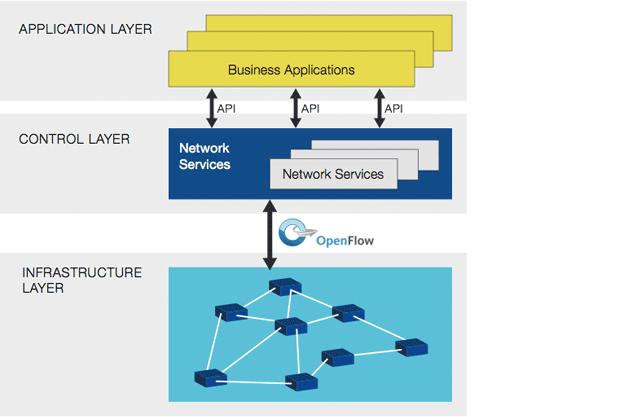
\includegraphics[width=20cm]{img/sdn-3layers.png}
   \caption{SDN 3 Layer Architecture}
   \label{fig:sdn3layer}
 \end{center}
 \end{figure}
\end{center}

SDN architecture is characterized by the following aspects:
\begin{itemize}
\item{\textbf{Open standards-based and vendor-neutral}}: Being implemented through open standards, SDN simplifies network design and operation. Instructions are provided by SDN controllers, which follow a particular set of open protocols and devices, instead of multiple, vendor-specific devices and protocols.
\item{\textbf{Directly programmable}}: Network control plane is directly programmable. This aspect is possible due to the fact that control planeis decoupled from forwarding plane.
\item{\textbf{Agile}}: Abstracting control from forwarding plane lets network administrators dynamically adjust network-wide traffic flow to meet particular needs of the network at each particular moment.
\item{\textbf{Centrally managed}}: Network intelligence is centralized in software-based SDN controllers. This kind of elements maintain a global view of the network topology. Network itself appears to applications and policy engines as a single, logical switch.
\item{\textbf{Programmatically configured}}: Network managers can configure, manage, secure, and optimize network resources through SDN very quickly via dynamic, automated SDN programs, which can be written themselves because the programs do not depend on proprietary software.
\end{itemize}
Previous detailed aspects make SDN technology to be one of the most recently boosting technologies, together with Cloud Computing and Big Data. Indeed, the increasing interests in all of them has also to do with the fact that all these technologies, together with Virtualization, are necessary linked between them.\\
\\
Next section shows how the market has increased in the last years, together with the big expectations that SDN tecnhology is supposed to have in the next years.

\subsection{SDN: Market share and expectations}

SDN is considered a boosting technology. In year 2013, the service-provider SDN market —hardware and software combined — was about \textbf{\$840 million in 2013} and is considered to grow to \textbf{\$15.6 billion in 2018}, according to a report released by ACG Research~\cite{SDN2018expectations00}.\\
\\
In this research, numbers don’t include the enterprise market, and apply only to service providers, including large-data-center owners such as Google and the big data centers of carriers such as NTT or AT\&T.\\
\\
Here’s how ACG’s 2018 forecast breaks down into the different sub-markets taking into account the different main areas of SDN deployment:

\begin{table}[H]
\footnotesize
\begin{center}
\begin{tabular}{|l|l|l|}
\hline
\textbf{SDN Submarket} & \textbf{Market expectation} \\ \hline
Data center	& \$3.3 billion \\ \hline
IP services	& \$4.2 billion \\ \hline
Metro networks &	\$4.3 billion \\ \hline
Core networks & \$3.8 billion  \\ \hline
\end{tabular}
\end{center}
\caption{SDN 2018 Sub-Market Expectations}
\label{tab:2018submarketexpectations}
\end{table}
The numbers reflect only “live” SDN deployments, i.e.: cases where service providers would use the technology, and not just installing it for future use.\\
\\
However, it must be remarked that expectations are even higher considering other reports. By mid 2013, market considered for year 2013 was about \$1.5 billion, and expectations for year 2018 was about \$35.5 billion according to a research by SDNCentral~\cite{SDN2018expectations01}.

\begin{center}
 \begin{figure}[H]
 \begin{center}
   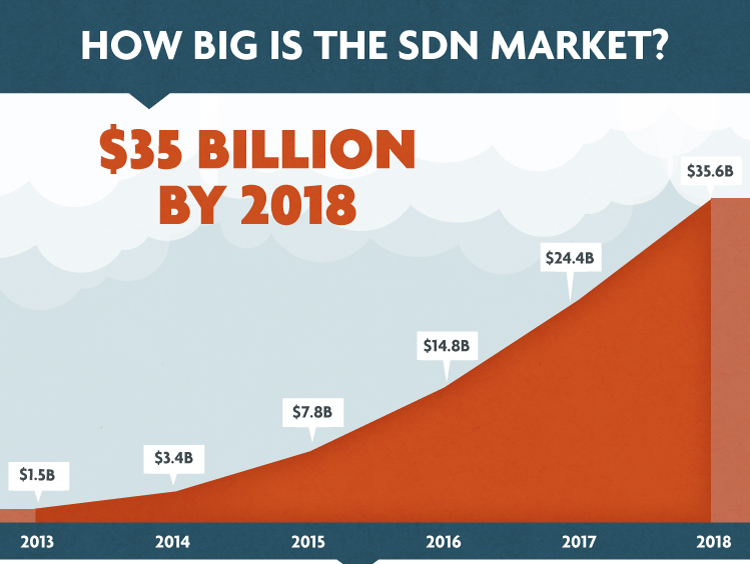
\includegraphics[width=15cm]{img/sdn_estimations_2018.png}
   \caption{SDN Market: 2018 SDNCentral estimations}
   \label{fig:sdn2018estimations}
 \end{center}
 \end{figure}
\end{center}

This last analysis and infographics doesn’t compare directly with previous one, as it wasn’t limited to service providers, and included SDN-ready equipment, sales that represent customers preparing for SDN even if they wouldn’t be using it immediately.\\
\\
Analyzing the data of this last report, a number of key takeaways must be highlighted:
\begin{enumerate}\itemsep0pt
 \item{The software-defined networking SDN market is expected to surpass \$35 billion in 2018}.
 \item{Adoption of SDN technology has accelerated in recent years from sales of \$10 million in 2007 to \$252 million in 2012}.
 \item{The emergence of the software-defined networking market is supported by growth in venture capital investment in SDN-focused companies}. Venture capital funding of SDN-related companies rose from \$10 million in 2007 to \$454 million in 2012.
\end{enumerate}

According to this report, the main three areas driving the rise in SDN are:
\begin{enumerate}\itemsep0pt
\item{Cloud Computing}
\item{Big Data}
\item{Mobility}
\end{enumerate}
Apart from pure SDN Market numbers, there are other aspects to consider. For example, the VC(Venture Capital) investment has grown, according to this report, from \$10 million in 2007 to \$454million in 2012.\\
\\
This report also considers that Networking Industry spending Percentage on SDN will rise from 2\% in 2013 to 40\% in 2014, with more than 220 companies by mid 2013, compared to the zero existing in 2009.\\
\\
Last, but not least, it must be remarked that up to more than \$1.5 billion has been invested in acquisitions of SDN related companies up to 2013, including the most remarkable one, the acquisition of Nicira Inc. by VMWare by July 2012, for approximately \$1.05 billion in cash plus approximately \$210 million of assumed unvested equity awards~\cite{VMWareAcquireNicira}.\\
\\
Far from giving a very detailed information on SDN market, this section has shown through all the numbers above how important is the SDN market and how important could be an Open Source Software Project such as OpenDaylight, which is in the end a key component in SDN deployment.

\section{NFV}
\label{sec:nfv}

Network Functions Virtualisation is a concept directly tied to Network Operators, as, normally, therir networks consist of a large and increasing variety of proprietary hardware and software applications that implement different functionality.\\
\\
To launch a new service on a Network Operator usually requires yet another different kind of hardware, meaning finding the space and power to accommodate these new equipment. As time goes by and Network Operator infrastructure grows, adding new appliances becoms more difficult, by the increasing costs of energy, capital investment challenges and, of course the rarity of skills necessary to design, integrate and operate these new equipment.\\
\\
Apart from that, end of life for hardware-based appliances is reached rapidly, requiring much of the integration and deploy cycle to be repeated with no revenue benefit in most of the cases. Besides this, hardware lifecycles are becoming shorter, due to the fact that technology and services innovation accelerates quicker up on time.

\subsection{What is NFV?}

As defined by \textbf{ETSI} in~\cite{ETSINFVDefinition} defines \textbf{Network Functions Virtualisation} as follows:
\begin{verbatim}
Network Functions Virtualisation aims to transform
the way that network operators architect
networks by evolving standard IT virtualisation
technology to consolidate many network equipment
types onto industry standard high volume servers,
switches and storage, which could be located in
Datacentres, Network Nodes and in the end user
premises.
\end{verbatim}
What NFV aims to get is, basically, homogenize the hardware of a Network Operator to basically three kind of standard generic use hardware. In particular, by the use of \textbf{High Volume Servers}, \textbf{High Volume Storage} and \textbf{High Volume Ethernet Switches}. Accomplishing this homogenization involves the implementation of \textbf{Network Functions} in software. This Network Functions must run on a range of industry standard server hardware, and can be moved to, or instantiated in, various locations in the network as required, without the need for installation of new equipment, at least, from a functional perspective.\\
\\
In the end, for Network Operators, NFV means migration of the different hardware specific nodes implementing different functionalities, such as DPI (Deep Packet Inspection), Firewalls, CDN (Content Delivery Network), Radio Access Network Nodes, Message Router, Carrier Grade NAT and/or any other network specfic functionality, which involve \textbf{Fragmented non-commodity hardware}, to Network Functions (also known as \textbf{Virtual Appliances}) running on previously defined Standard High Volume hardware.

\begin{center}
 \begin{figure}[H]
 \begin{center}
   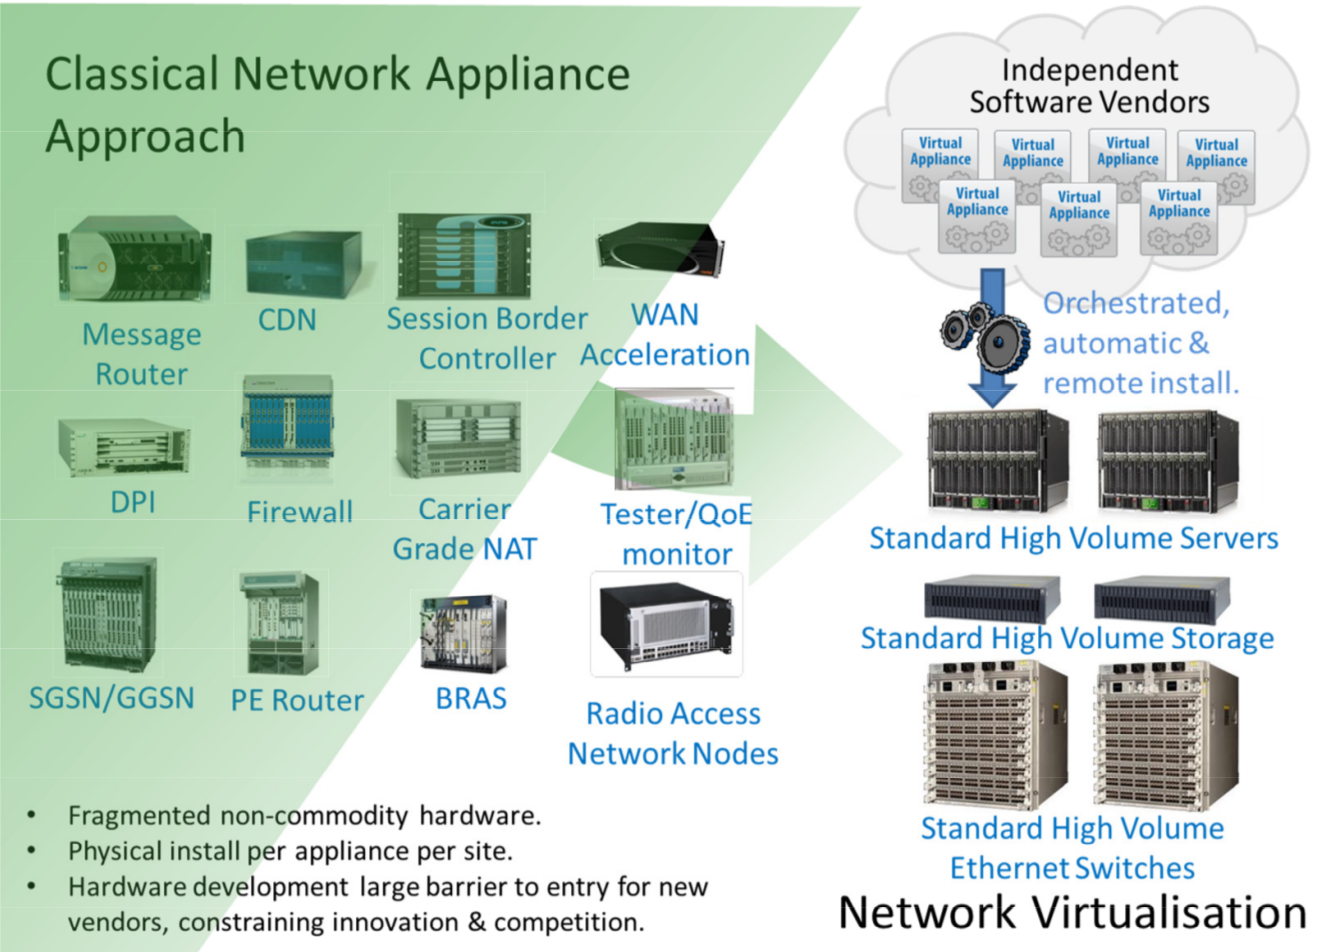
\includegraphics[width=15cm]{img/nfv-etsi-01.png}
   \caption{Vision of Network Functions Virtualisation}
   \label{fig:nfv_vision}
 \end{center}
 \end{figure}
\end{center}

\subsection{SDN/NFV relationship}

Network Functions Virtualisation is highly complementary to Software Defined Networking (SDN), as recognized by \textbf{ETSI} in~\cite{ETSINFVDefinition}. However NFV is not dependent on SDN (or vice-versa). NFV can be implemented without a SDN being required, although the \textbf{both solutions can be combined and potentially greater value accrued}.\\
\\
Network Functions Virtualisation goals can be achieved using non-SDN mechanisms, relying on the techniques currently in use in many operators. But approaches relying on the separation of the control and data forwarding planes as proposed by SDN can enhance performance, simplify compatibility with existing deployments, and facilitate operation and maintenance procedures.\\
\\
Network Functions Virtualisation is able to support SDN by providing the infrastructure upon which the SDN software can be run. Furthermore, Network Functions Virtualisation aligns closely with the SDN objectives to use commodity servers and switches.

\begin{center}
 \begin{figure}[H]
 \begin{center}
   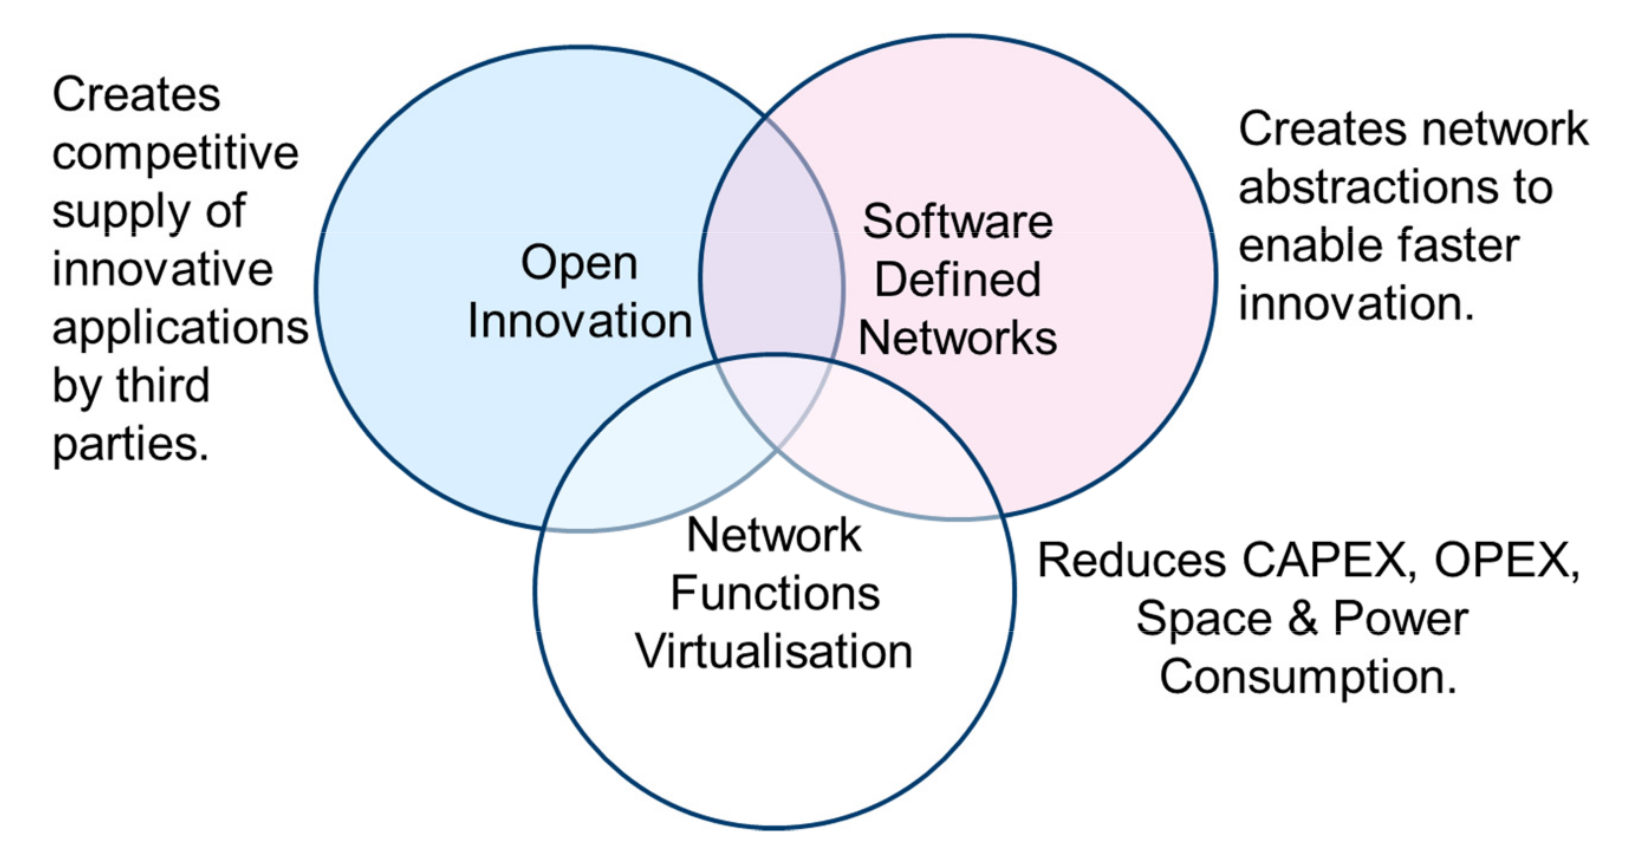
\includegraphics[width=15cm]{img/sdn-nfv-relationship-00.png}
   \caption{Network Functions Virtualisation relationship with SDN}
   \label{fig:nfv_sdn_relationship}
 \end{center}
 \end{figure}
\end{center}
ETSI intends to work closely with organisations progressing work on SDN such as the Open Networking Foundation (ONF) whose work is specifically taken into account by SDN to achieve common goals.

\subsection{NFV benefits}

Taking into account previous sections, where NFV concept has been detailed, an analysis of the main benefits of the migration of the Network Operators to this kind of infrastructure based on Virtual Appliances running on common High Volume Hardware. ETSI~\cite{ETSINFVDefinition} defines next \textbf{benefits} for a Network Operator taking into account migration to Network Functions Virtualisation:

\begin{itemize}\itemsep0pt
 \item{\textbf{Reduced equipment cost}}. Basically, by exploiting the economies of scale of the IT industry.
 \item{\textbf{Increased velocity of Time to Market}}. By minimising the network operator cycle of innovation.
 \item{\textbf{Reduction of development costs and time to market}}. Motivated by a more efficient test and integration, and the possibility of running production, test and reference facilities on the same infrastructure.
 \item{\textbf{More innovation due to openness}}. Motivated by Open Virtual Appliance market where small players and academia can bring new services.
 \item{\textbf{Optimizing network configuration and/or topology}}. This optimization can be performed in near real time based on the actual traffic/mobility patterns and service demand.
 \item{\textbf{Reduced energy consumption}}. By exploiting power management features in standard servers and storage hardware.
 \item{\textbf{Improved Operational Efficiency}}. Taking advantage of the uniformity of the physical network platform:
 \begin{itemize}\itemsep0pt
    \item{IT orchestration mechanisms provide automated installation}.
    \item{Eliminating the need for application-specific hardware}. The skills base across the industry for operating standard high volume IT servers is much larger and less fragmented.
    \item{Reduction in variety of equipment for planning and provisioning}.
    \item{Option to temporarily repair failures by automated re-configuration}.
    \item{The potential to gain more efficiency between IT and Network Operations}.
    \item{The potential to support in-service software upgrade}.
 \end{itemize}
\end{itemize}

On this chapter, a first introduction to the \textbf{OpenDaylight Open Source Project} has been presented. Apart from that, main technologies involved in this project, \textbf{SDN} and \textbf{NVF} have been introduced as well. On next sections, it will be studied in depth other aspects of the project, focusing on those areas having to do with Open Source nature of the project.

\chapter{OpenDaylight: Legal Aspects}
\label{chap:odllegal}

\section{OpenDaylight License: EPLv1.0}
\label{sec:odllicense}

OpenDaylight project has been released under EPL (Eclipse Public License)-v1.0~\cite{EPLv1}. This license, that was launched in February 2004, is considered an \textbf{Open Source Software License} due to basically two reasons:
\begin{enumerate}\itemsep0pt
 \item {It guarantees the ``Four Freedoms'' that Open Source must guarantee}:
  \begin{itemize}\itemsep0pt
   \item{Freedom to use}.
   \item{Freedom to inspect}.
   \item{Freedom to copy and redistribute copies}.
   \item{Freedom to modify and redistribute modified versions}.
  \end{itemize}
 \item {It is considered also \textbf{Open Source/Free Software} due to the fact that the two main groups having to do with this kind of softare recognizes the license to be Open Source/Free Software}:
  \begin{itemize}\itemsep0pt
   \item{\textbf{Open Source Initiative}~\cite{OpenSourceInitiiative}}. This corporation recognizes EPLv1.0 not only among the ones considered to be an \textbf{Open Source license}, but also \textbf{one of the most popular ones}~\cite{OSILicenses}.
   \item{\textbf{Free Software Foundation}~\cite{FreeSoftwareFoundation}}. This nonprofit organization recognizes this license to be a \textbf{Free Software license}, although \textbf{EPLv1.0 is not compatible with GNU GPL}~\cite{FSFLicense}.
  \end{itemize}
\end{enumerate}
Taking into consideration that EPLv1.0 is Open Source, a deeper anaylisis of this license must be performed. Before analysing which kind of Open Source software license is EPLv1.0, a classification of the different kind of Open Source licenses should be performed. However, before doing such analysis, a concept related to Open Source license, which is \textbf{Copyleft}, must be introduced. According to FSF~\cite{FSFCopyleft}:
\begin{verbatim}
Copyleft is a general method for making a program
(or other work) free, and requiring all modified
and extended versions of the program to be free as well.
\end{verbatim}
However, this definition is not as concrete as it should. Although the term ``Copyleft'' was defined by FSF, OSI defines the concept in a much more understandable way~\cite{OSICopyleft}:
\begin{verbatim}
"Copyleft" refers to licenses that allow derivative works
but require them to use the same license as the original work.
For example, if you write some software and release it under
the GNU General Public License (a widely-used copyleft license),
and then someone else modifies that software and distributes
their modified version, the modified version must be licensed under
the GNU GPL too.
\end{verbatim}
Taking into consideration previous concept, according to the kind of licenses and if they are copyleft licenses or not, it is usual to follow this \textbf{classification regarding Open Source Software Licenses}:

\begin{itemize}\itemsep0pt
 \item{\textbf{Minimalistic/Academic Licenses}}: These kind of \textbf{No Copyleft} licenses are the most simple ones. \textbf{None of them has Patent Software clauses}, and they \textbf{rarely mean uncompatibilities} with other kind of licenses. This kind of license is normally very well considered (for both parts, open source and privative industry). They usually contain a \textbf{No warranty" clause}, and normally have \textbf{no restrictions}. They usually suppose \textbf{no legal complexity}. The most popular of this kind of licenses are:
   \begin{itemize}\itemsep0pt
    \item{BSD License}.
    \item{ISC License}.
    \item{MIT License}.
   \end{itemize}
 \item{\textbf{Permissive Licenses}}: This kind of \textbf{No Copyleft} licenses are similar to the academic ones, but they normally include some kind of restriction or punctualisation. This kind of restriction is normally related to \textbf{Patent Software clauses}. They \textbf{rarely mean uncompatibilities} with other kind of licenses, \textbf{although there are exceptions}. Among this kind of licenses, \textbf{the most popular one is Apache License}.
 \item{\textbf{Weak Copyleft Licenses}}: This kind of \textbf{Weak Copyleft} licenses contain copyleft clauses with certains limitations. They normally define that \textbf{not all derivative works must the copyleft license}. Derivative works inherits or not the license often depending on the manner in which it was derived. They are normally considered \textbf{Copyleft oriented to just source files}. The most popular of this kind of licenses are~\cite{FSFLicense}:
   \begin{itemize}\itemsep0pt
    \item{Mozilla Public License}.
    \item{Common Public License}.
    \item{\textbf{Eclipse Public License}}.
   \end{itemize}
 \item{\textbf{Copyleft Licenses}}: This kind of \textbf{Copyleft} licenses contain \textbf{strong clauses related to redistribution of derivative works}. This kind of licensing was first introduce by FSF, and is not well considered because of its \textbf{``viral character''}. The most popular license of this type is \textbf{GNU Generic Public License (GPL)}.
\end{itemize}
Once described the classification of Open Source licenses, it has been asserted that EPLv1.0 is classified as a \textbf{Weak Copyleft} license, as recognized by FSF~\cite{FSFEPL}. But, apart from that, inspecting the EPLv1.0 license, it can be found that \textbf{there is a possibility to distribute software under on its own license agreement~\cite{EPLv1}}, when distributing ``object code'':
\begin{verbatim}
3. REQUIREMENTS
A Contributor may choose to distribute the Program in
object code form under its own license agreement,
....
When the Program is made available in source code form:
a) it must be made available under this Agreement; and
b) a copy of this Agreement must be included with each copy
of the Program.
\end{verbatim}
As demonstrated above, there are some conditions in the license that allow this software to be distributed under other kind of license. However, if distributing source code, distribution must be performed under same agreement. \textbf{This kind of clauses are the ones that make this kind of licenses to be known ``Copyleft oriented to source files''}.\\
\\
NOTE (CHANGE): Maybe deeper information on Eclipse Public License in next URL link can be considered: http://oss-watch.ac.uk/resources/epl\\
\\
Once EPLv1.0 license has been analyzed and classified, it must be analyzed \textbf{which reasons make OpenDaylight Open Source project} to use this kind of license. In the FAQ section of OpenDaylight Open Source project, next statement appears~\cite{OpenDaylightFAQ5}:

\begin{verbatim}
5. What license will the project use? Why was that decision made?

OpenDaylight is structured and governed using open source best
practices and is licensed under the Eclipse Public License-v1.0
(EPL), which is a common choice for Java-based projects. The EPL
is an approved open source license by the Open Source Initiative
and considered a free software license by the Free Software
Foundation. The license choice of EPL maximizes OpenDaylight’s
license compatibility with the large ecosystem of libraries and
3rd party components that have already been released under the EPL
license. Where necessary the Board may approve exceptions for other
licenses.
\end{verbatim}
Basically, the reasons for using this kind of license are basically three:
\begin{itemize}
 \item{\textbf{Open Source/Free Software license}}. Being recognized by both OSI and FSF, this license is suitable into the structured and governance bylaws of the project having to do with its Open nature and commitment to the Open Source movement.
 \item{\textbf{Java-based project}}. EPLv1.0 is a common license for Java-based projects. Being \textbf{developed in Java programming language primarily}, OpenDaylight Open Source project fits quite well into this kind of license, as other projects written in Java do, as, for instance, Eclipse IDE.
 \item{\textbf{3rd party libraries/components compatibility}}. Last, but not least, Board in OpenDaylight decided that \textbf{EPLv1.0 license fits better in terms of compatibility with 3rd party components and libraries used} inside the project compared to other kind of licenses. Examples of 3rd parties used in OpenDaylight Open Source project are Java programming language, Maven, Open vSwitch or Open Flow Java implementation.
 \item{\textbf{Avoid licensing fragmenation}}. Using this kind of ``Weak Copyleft'' license helps on avoiding licensing fragmentation for derivative works/forks/spinoffs. A more detailed information on how fragmentation is avoided appears on Section~\ref{sec:otherlicensebylaws}.
\end{itemize}
Up to this point, EPLv1.0 and OpenDaylight Open Source project to use this license have been analysed. In next section, other legal considerations and Bylaws will be studied in order to clarify other important issues that are considered inside OpenDaylight Open Source project to be important as well.

\section{Other Licensing Considerations}
\label{sec:otherlicenseconsiderations}

On previous section EPLv1.0 license and its application to the OpenDaylight Open Source pr oject were studied. However, there are \textbf{other licensing considerations} to take into account by the project and its Governance Board.\\
\\
For this reason, having a look at the FAQ of OpenDaylight Open Source Project~\cite{OpenDaylightFAQ}, other legal considerations must be taken into account:

\begin{verbatim}
8. Will all development be done in the open?
All OpenDaylight source code development will be done
in the open. Some contributors or companies may choose
to incubate and develop code internally and then contribute
it openly later, which is fine as well, but the core project
code will all be developed in the open for everyone to see
and use under a standard OSI-approved EPL open source license.
\end{verbatim}
Previous statement tries to perform as a \textbf{declaration of intent} by the project Governance. In particular, it tries to clarify the intention of perform development of the core project with an Open Source licensing scheme, \textbf{clarifying the intention to use EPL Open Source license} as a general rule to guarantee open development.

\begin{verbatim}
17. Will the products developed on the framework also be
open source?
This is the sole discretion of each company. The intent of
OpenDaylight is to employ collaborative, open source development
to build and support an open source framework and codebase on top
of which commercial products and services can be built. How each
vendor adopts OpenDaylight and commercializes their own products
will be an individual business decision for them, subject to the
Eclipse Public License.
\end{verbatim}
With previous statement, the OpenDaylight Open Source Project Governance tries to clarify the discretion of each company to perform \textbf{whichever commercial actions they consider}, taking into account the Eclipse Public License and the different statements appearing on it. Far from being commercially agnostic, this statement is a nod to empower companies to use this Open Source project as a base to commercialize products and services.

\begin{verbatim}
19. How will OpenDaylight prevent fragmentation?

Many open source projects eventually see forks or spinoffs
from the original codebase. Experimentation and innovation
off of an open source codebase is common and encouraged.
However, long term the open governance and open technical
decision making structure employed by the OpenDaylight
project should help minimize the need to do any significant
fragmentation from the core project codebase.
Further, OpenDaylight employs an OSI approved open source
license. The EPL requires any distributed modifications to
the program also be licensed under the EPL. For more
information on the EPL, see the Eclipse EPL FAQ.
\end{verbatim}
\noindent Previous statement is a clarification about the \textbf{decission to use EPL} to minimize forks of the original codebase. This license usage does not guarantee forks/spinoffs of the project are not taking place, but, at least, guarantees them to be Open Source if the source code is modified and wants to be distributed. In next section, \textbf{Bylaws of OpenDaylight Open Source project} will be summarized. Far from being analysed in a deep basis, the most important statements in the project bylaws are to be enumerated in order to \textbf{clarify those legal statements} that must be taken into consideration.

\section{Bylaws}
\label{sec:bylaws}
Adopted by July 28, 2014, OpenDaylight Project Inc. contains a set of thirteen articles to clear up all the different issues from a Legal and/or Governance perspective. The document, known as ``Second Amended And Restated By-Laws''~\cite{OpenDaylightBylaws}, is summarized in Appendix~\ref{chap:appendix_bylaws}, and define a complete legal statement that considers several aspects having to do with:
\begin{enumerate}\itemsep0pt
 \item{\textbf{Name, Purpose and Offices}}
 \item{\textbf{Members}}
 \item{\textbf{Actions of Members}}
 \item{\textbf{Directors}}
 \item{\textbf{Executive Committee and Other Committees}}
 \item{\textbf{Officers}}
 \item{\textbf{Notices}}
 \item{\textbf{Indemnification}}
 \item{\textbf{Books And Records}}
 \item{\textbf{Certain Transactions}}
 \item{\textbf{Grants, Contracts and Loans}}
 \item{\textbf{General Provisions}}
 \item{\textbf{Antitrust Compliance}}
 \item{\textbf{Ammendments}}
\end{enumerate}

\chapter{OpenDaylight: Governance and Community Management}
\label{chap:odlcommunity}

\chapter{OpenDaylight: Technical Aspects}
\label{chap:odltechnical}

\chapter{OpenDaylight: Economic Aspects}
\label{chap:odleconomic}

\chapter{OpenDaylight: Project Evaluation}
\label{chap:odlprojeval}

%%%%%%%%%%%%%%%%%%%%%%%%%%%%%%%%%%%%%%

\chapter{Conclusions}
\label{chap:conclusions}

%%%%%%%%%%%%%%%%
% Review goals and objectives

\section{Evaluation}
\label{sec:evaluation}

%%%%%%%%%%%%%%%%%%%%%%%%%%%%%%%%%%%%%%

Review goals and objectives

%%%%%%%%%%%

\section{Lessons learned}
\label{sec:lessons}

\subsection{Lesson 1}
\begin{itemize}
 \item Explain here what anybody may learn from this document
\end{itemize}

\subsection{What I learned}
\begin{itemize}
 \item Explain what you learned writing this document
\end{itemize}

\subsection{Knowledge and skills acquired in the M.Sc. studies that helped me on
this work}
\begin{itemize}
 \item You can go subject by subject, explained in which aspects helped
you to do/write this project
 \item Or just mention only the main aspects/subjects

\end{itemize}

\section{Future work}
\label{sec:future}

\subsection{More on...}

If there is any aspect that is not fully covered, explain how it could be
better covered.

\subsection{Other aspects}

See the section about ``Scope'' and explain here other aspects that you didn't
cover but it could be nice to work on.


\subsection{Other focuses}

For example study similar projects, or apply other tools to do the same work.

%%%%%%%%%%%%%%%%%%%%%%%%%%%%%%%%%%%%%
\appendix

%%%%%%%%%%%%%%%%%%%%%%%%%%%%%%%%%%%%%%
\chapter{Bylaws Summary}
\label{chap:appendix_bylaws}
\begin{table}[H]
  \begin{center}
    \begin{tabular}{ | p{4cm} | p{11cm} | }
    \toprule
    \multicolumn {2}{|c|}{\textbf{Article I: Name, Purpose and Offices}} \\
    \multicolumn {2}{|c|}{This Article focuses on some legal aspects such as the name of the company, the offices or} \\
    \multicolumn {2}{|c|}{the purpose and non-profit status of the project} \\
    \hline
    \textbf{Section} & \textbf{Description} \\
    \hline
    1.1: Name & Name of the corporation will be “OpenDaylight Project, Inc.”, referred to in these By-laws as the “ODP” \\
    \hline
    1.2: Principal Office & Located at San Francisco, CA 94110.  The Board of Directors of the ODP (the “Board”) is hereby granted full power and authority to change its principal office \\
    \hline
    1.3: Other Offices & Branch or subordinate offices may at any time be established by the Board at any place or places \\
    \hline
    1.4: Purpose & ... The primary purpose of the ODP (collectively, “the Purpose”) is to (a) advance the creation, evolution, promotion, and support of an open source software defined network and network functions virtualization software platform ... \\
    \hline
    1.5: Nonprofit Status & (a) The ODP is organized and shall be operated as a non-stock, not for profit membership corporation ... (b) The Board may, in its sole discretion, elect to seek exemption from Federal taxation ...\\
    \bottomrule
    \end{tabular}
    \caption{OpenDaylight Bylaws Summary: Article I}
    \label{tab:odlbylaws-art01}
  \end{center}
\end{table}

\begin{table}[H]
  \begin{center}
    \begin{tabular}{ | p{4cm} | p{11cm} | }
    \toprule
    \multicolumn {2}{|c|}{\textbf{Article II: Members}} \\
    \multicolumn {2}{|c|}{This Article focuses on the different kind of members} \\
    \multicolumn {2}{|c|}{the conditions of membership} \\
    \hline
    \textbf{Section} & \textbf{Description} \\
    \hline
    2.1: Classes of Membership & Platinum Members, Strategic End-User Members, Gold Members, Silver Members, Individual Committer Members, and Associate Members. Additional classes of voting and non-voting members may be created in the future...\\
    \hline
    2.2: Conditions of Membership & Any association, partnership, organization, governmental agency, company, corporation, academic entity, or non-profit entity (or individual, solely with respect to Individual Committer Members or Associate Members) ...\\
    \hline
    2.3 to 2.8: Privileges & These sections reflect the privileges of being Platinum Member, Strategic End-User Member, Gold Member, Silver Member, Individual Committer or Associate Member\\
    \bottomrule
    \end{tabular}
    \caption{OpenDaylight Bylaws Summary: Article II}
    \label{tab:odlbylaws-art02}
  \end{center}
\end{table}

\begin{table}[H]
  \begin{center}
    \begin{tabular}{ | p{4cm} | p{11cm} | }
    \toprule
    \multicolumn {2}{|c|}{\textbf{Article III: Actions of Members}} \\
    \multicolumn {2}{|c|}{This Article focuses on the different kind of actions} \\
    \multicolumn {2}{|c|}{that members can carry out} \\
    \hline
    \textbf{Section} & \textbf{Description} \\
    \hline
    3.1: Action Without Meeting & Any action required or permitted to be taken by the Members, ... or at any meeting of a Member Committee, Working Group ..., may be taken without prior notice and without an in-person vote, if a consent in writing, setting forth the action to be taken, shall be signed by Members ...\\
    \hline
    3.2: Nomination and Election Procedures & Subject to the provisions of Section 4.3, the Board shall establish reasonable nomination and election procedures given the nature, size, and operations of the ODP, including a reasonable means for Members of appropriate classes to nominate a person for election as a Director.\\
    \bottomrule
    \end{tabular}
    \caption{OpenDaylight Bylaws Summary: Article III}
    \label{tab:odlbylaws-art03}
  \end{center}
\end{table}

\begin{table}[H]
  \begin{center}
    \begin{tabular}{ | p{4cm} | p{11cm} | }
    \toprule
    \multicolumn {2}{|c|}{\textbf{Article IV: Directors}} \\
    \multicolumn {2}{|c|}{This Article focuses on the different kind of actions} \\
    \multicolumn {2}{|c|}{that members can carry out} \\
    \hline
    \textbf{Section} & \textbf{Description} \\
    \hline
    4.1: Powers; Voting & ... The Board may exercise all powers of the ODP and do all such lawful acts and things as are not by statute or by the Certificate of Incorporation or by these By-laws directed ...\\
    \hline
    4.2: Number of Directors & Subject to Section 4.4, the total number of Directors shall be at least one and not more than two (2) times the number of Platinum Members ...\\
    \hline
    4.3:  Nomination and Election & Each Platinum Member ... shall be entitled individually to appoint one Director ... (b) Each Strategic End-User Member (while remaining in good standing) shall be entitled individually to appoint one Director ... (c) Each Gold Member ... shall have the right to vote, together with the other Gold Members as a class, to elect a number of Directors equal to the number of Gold Members then in good standing divided by three (3) ... (d) Each Silver member ... shall have the right to vote, together with the other Silver Members as a class, to elect one (1) Director. \\
    \hline
    4.4: Enlargement or Reduction & ... the number of Directors, the persons eligible to become Directors and the classes of Members eligible to appoint, elect and/or nominate Directors may be amended at any time by a Super Majority Vote (as defined in Section 4.10(.b)) of the Board.\\
    \hline
    \bottomrule
    \end{tabular}
    \caption{OpenDaylight Bylaws Summary: Article III}
    \label{tab:odlbylaws-art03}
  \end{center}
\end{table}


\chapter{Second Appendix}

%%%%%%%%%%%%%%%%
% BIBLIOGRAPHY %
%%%%%%%%%%%%%%%%

\bibliographystyle{alpha}
\bibliography{bibliography}
\label{Bibliography}
\end{document}
